% sections/dsl_specification.tex

\section{Programmable Neural-Symbolic Configuration Language}
\label{sec:dsl}

While the YAML configuration format described in preceding sections is sufficient for direct human authorship, it conflates two concerns: the \emph{logical specification} of routing policy (signals, decisions, plugins) and the \emph{deployment target} (flat YAML, Kubernetes CRDs, Helm charts).
We introduce a programmable configuration language---the instruction set of the neural-symbolic inference engine (formalized in \Cref{sec:disc_agent})---that separates these concerns, providing a concise, human-readable, and machine-parseable surface syntax for routing policies that compiles to multiple deployment targets through a shared internal representation.

\subsection{Design Goals}

The DSL is designed around four principles:

\begin{enumerate}
  \item \textbf{Conciseness}: Routing policies should read as close to natural language as possible, minimizing syntactic noise relative to YAML.
  \item \textbf{Type safety}: Signal references in Boolean expressions are resolved at compile time; undefined or misspelled signal names produce diagnostics before deployment.
  \item \textbf{Multi-target emission}: A single DSL source compiles to flat YAML (for local development), Kubernetes \texttt{SemanticRouter} CRDs (for operator-based deployment), or Helm \texttt{values.yaml} (for chart-based deployment).
  \item \textbf{Round-trip fidelity}: An existing \texttt{RouterConfig} can be \emph{decompiled} back to DSL source, enabling migration from YAML to DSL and ``round-trip'' editing workflows.
\end{enumerate}

\subsection{Concrete Syntax}
\label{sec:dsl_syntax}

The DSL defines five top-level block types: \texttt{SIGNAL}, \texttt{ROUTE}, \texttt{PLUGIN}, \texttt{BACKEND}, and \texttt{GLOBAL}.
\Cref{fig:dsl_example} shows a representative configuration.

\begin{figure}[!htbp]
\centering
\footnotesize
\begin{verbatim}
SIGNAL domain math { mmlu_categories: ["math"] }
SIGNAL keyword urgent { operator: "any", keywords: ["urgent","asap"] }

PLUGIN safe_pii pii { enabled: true, pii_types_allowed: [] }

ROUTE math_route (description = "Math") {
  PRIORITY 100
  WHEN domain("math")
  MODEL "qwen2.5:3b" (reasoning = true, effort = "high")
  PLUGIN safe_pii
}
ROUTE urgent_ai {
  PRIORITY 200
  WHEN keyword("urgent") AND NOT domain("math")
  MODEL "qwen3:70b" (reasoning = true),
        "qwen2.5:3b" (reasoning = false)
  ALGORITHM confidence { threshold: 0.5 }
}

BACKEND vllm_endpoint ollama { address: "127.0.0.1", port: 11434 }
GLOBAL { default_model: "qwen2.5:3b", strategy: "priority" }
\end{verbatim}
\caption{A representative DSL configuration defining two signals, a reusable plugin template, two routes with Boolean decision logic, a backend endpoint, and global settings.}
\label{fig:dsl_example}
\end{figure}

Each \texttt{SIGNAL} block declares a named signal of a specific type (one of 12 supported types: \texttt{keyword}, \texttt{embedding}, \texttt{domain}, \texttt{fact\_check}, \texttt{user\_feedback}, \texttt{preference}, \texttt{language}, \texttt{context}, \texttt{complexity}, \texttt{modality}, \texttt{authz}, \texttt{jailbreak}, \texttt{pii}).
Each \texttt{ROUTE} block defines a decision with a priority, a Boolean \texttt{WHEN} clause over signal references, one or more model references with optional per-model parameters (reasoning mode, effort level, LoRA adapter, weight), an optional selection algorithm, and zero or more plugin attachments.
\texttt{PLUGIN} blocks at the top level define reusable templates that routes reference by name; inline plugin blocks within routes define route-specific configurations.

\subsection{Grammar and Parsing}
\label{sec:dsl_grammar}

The lexer and parser are implemented using the \texttt{participle} parser-generator library~\cite{participle2024}.
The lexer defines 12 token classes (identifiers, integers, floats, strings, booleans, braces, parentheses, brackets, colon, comma, equals, comments) via regular expressions.
The parser uses a PEG-style grammar with lookahead~3 to resolve ambiguities between signal references and other identifier uses.

The Boolean expression grammar for \texttt{WHEN} clauses follows standard precedence:

\begin{align}
  \textit{BoolExpr} &::= \textit{AndTerm} \;(\texttt{OR}\; \textit{AndTerm})^* \label{eq:bool_or} \\
  \textit{AndTerm} &::= \textit{Factor} \;(\texttt{AND}\; \textit{Factor})^* \label{eq:bool_and} \\
  \textit{Factor} &::= \texttt{NOT}\; \textit{Factor} \mid \texttt{(}\;\textit{BoolExpr}\;\texttt{)} \mid \textit{SignalRef} \label{eq:bool_factor} \\
  \textit{SignalRef} &::= \textit{type}\;\texttt{(}\;\textit{``name''}\;\texttt{)} \label{eq:signal_ref}
\end{align}

This grammar is parsed into a recursive AST (\texttt{BoolAnd}, \texttt{BoolOr}, \texttt{BoolNot}, \texttt{SignalRefExpr} nodes) that the compiler flattens into the \texttt{RuleCombination} tree consumed by the decision engine (\Cref{sec:decision_engine}).
\Cref{fig:bool_ast} illustrates the AST for a representative Boolean expression.

\begin{figure}[!ht]
  \centering
  \resizebox{\linewidth}{!}{%
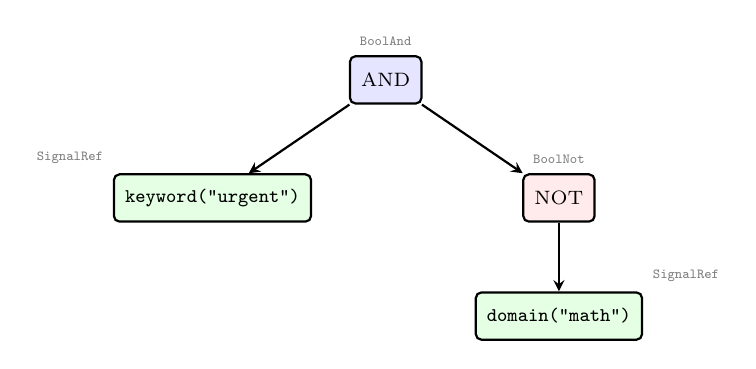
\begin{tikzpicture}[
    tnode/.style={rectangle, draw, thick, rounded corners=2pt,
                  minimum height=0.6cm, align=center, inner sep=4pt, font=\scriptsize},
    arr/.style={->, >=stealth, thick},
    lbl/.style={font=\tiny, text=gray},
  ]

  % Root: AND
  \node[tnode, fill=blue!10] (and) at (0, 0) {AND};
  \node[lbl, anchor=south] at (and.north) {\texttt{BoolAnd}};

  % Left child: keyword("urgent")
  \node[tnode, fill=green!10] (kw) at (-2.2, -1.5) {\texttt{keyword("urgent")}};
  \node[lbl, anchor=south east] at (kw.north west) {\texttt{SignalRef}};

  % Right child: NOT
  \node[tnode, fill=red!8] (not) at (2.2, -1.5) {NOT};
  \node[lbl, anchor=south] at (not.north) {\texttt{BoolNot}};

  % NOT's child: domain("math")
  \node[tnode, fill=green!10] (dom) at (2.2, -3.0) {\texttt{domain("math")}};
  \node[lbl, anchor=south west] at (dom.north east) {\texttt{SignalRef}};

  % Edges
  \draw[arr] (and) -- (kw);
  \draw[arr] (and) -- (not);
  \draw[arr] (not) -- (dom);

  \end{tikzpicture}%
}
  \caption{Boolean expression AST for \texttt{WHEN keyword("urgent") AND NOT domain("math")}. Each leaf is a \texttt{SignalRefExpr} referencing a named signal; internal nodes are Boolean operators (\texttt{BoolAnd}, \texttt{BoolNot}). The compiler flattens this tree into a \texttt{RuleCombination} structure for the decision engine.}
  \label{fig:bool_ast}
\end{figure}

Error recovery is block-granular: if parsing a top-level block fails, the parser splits the input at block boundaries and attempts to parse remaining blocks independently, accumulating partial results alongside error diagnostics.
This enables IDE-like incremental feedback during authoring.

\subsection{Compilation Pipeline}
\label{sec:dsl_compilation}

The compilation pipeline (\Cref{fig:dsl_pipeline}) transforms DSL source through four stages:

\begin{enumerate}
  \item \textbf{Lexing}: The source is tokenized into a stream of typed tokens with position tracking for diagnostic reporting.
  \item \textbf{Parsing}: The token stream is parsed into a \emph{raw parse tree} (participle-generated structs), then lowered to a \emph{resolved AST} (\texttt{Program} $\to$ \texttt{SignalDecl}, \texttt{RouteDecl}, \texttt{PluginDecl}, \texttt{BackendDecl}, \texttt{GlobalDecl}) with desugared values and resolved positions.
  \item \textbf{Compilation}: The AST is compiled to the internal \texttt{RouterConfig} structure. This involves: (a) mapping each \texttt{SIGNAL} block to the appropriate signal configuration (keyword rules, embedding rules, domain categories, etc.); (b) flattening the Boolean expression tree in each \texttt{WHEN} clause into a \texttt{RuleCombination} tree with \texttt{AND}/\texttt{OR}/\texttt{NOT} operators; (c) resolving plugin references against top-level templates with field-level merge semantics (route-local fields override template defaults); and (d) mapping \texttt{BACKEND} blocks to endpoint, provider profile, embedding model, or semantic cache configurations based on the backend type keyword.
  \item \textbf{Emission}: The \texttt{RouterConfig} is serialized to one of three target formats.
\end{enumerate}

\begin{figure*}[!ht]
  \centering
  \resizebox{\linewidth}{!}{%
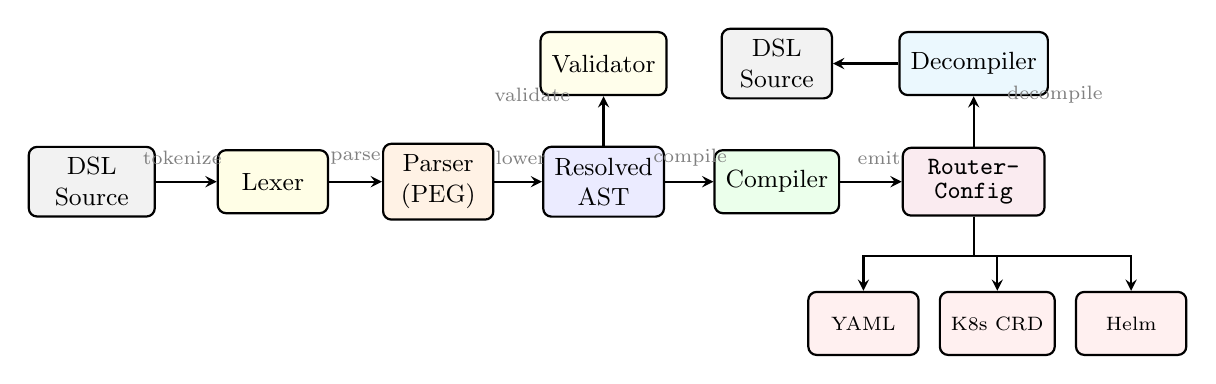
\begin{tikzpicture}[
    box/.style={rectangle, draw, thick, rounded corners=3pt,
                minimum height=0.8cm, align=center, inner sep=4pt, font=\small},
    arr/.style={->, >=stealth, thick},
    lbl/.style={font=\scriptsize, text=gray},
  ]

  % Source
  \node[box, fill=black!5, minimum width=1.6cm] (src) at (0, 0) {DSL\\Source};

  % Lex
  \node[box, fill=yellow!10, minimum width=1.4cm] (lex) at (2.3, 0) {Lexer};

  % Parse
  \node[box, fill=orange!10, minimum width=1.4cm] (parse) at (4.4, 0) {Parser\\(PEG)};

  % AST
  \node[box, fill=blue!8, minimum width=1.4cm] (ast) at (6.5, 0) {Resolved\\AST};

  % Compile
  \node[box, fill=green!8, minimum width=1.5cm] (comp) at (8.7, 0) {Compiler};

  % RouterConfig
  \node[box, fill=purple!8, minimum width=1.8cm] (cfg) at (11.2, 0) {\texttt{Router-}\\[-2pt]\texttt{Config}};

  % Emitters (branching)
  \node[box, fill=red!6, font=\scriptsize, minimum width=1.4cm] (eyaml) at (9.8, -1.8) {YAML};
  \node[box, fill=red!6, font=\scriptsize, minimum width=1.4cm] (ecrd) at (11.5, -1.8) {K8s CRD};
  \node[box, fill=red!6, font=\scriptsize, minimum width=1.4cm] (ehelm) at (13.2, -1.8) {Helm};

  % Decompiler (reverse)
  \node[box, fill=cyan!8, minimum width=1.5cm] (decomp) at (11.2, 1.5) {Decompiler};
  \node[box, fill=black!5, minimum width=1.4cm] (dsout) at (8.7, 1.5) {DSL\\Source};

  % Validator
  \node[box, fill=yellow!8, minimum width=1.4cm] (valid) at (6.5, 1.5) {Validator};

  % Arrows
  \draw[arr] (src) -- (lex);
  \draw[arr] (lex) -- (parse);
  \draw[arr] (parse) -- (ast);
  \draw[arr] (ast) -- (comp);
  \draw[arr] (comp) -- (cfg);

  \draw[arr] (cfg.south) -- ++(0,-0.5) -| (eyaml.north);
  \draw[arr] (cfg.south) -- ++(0,-0.5) -| (ecrd.north);
  \draw[arr] (cfg.south) -- ++(0,-0.5) -| (ehelm.north);

  \draw[arr] (cfg.north) -- (decomp.south);
  \draw[arr] (decomp.west) -- (dsout.east);

  \draw[arr] (ast.north) -- (valid.south);

  % Labels
  \node[lbl] at (1.15, 0.3) {tokenize};
  \node[lbl] at (3.35, 0.3) {parse};
  \node[lbl] at (5.45, 0.3) {lower};
  \node[lbl] at (7.6, 0.3) {compile};
  \node[lbl] at (10.0, 0.3) {emit};
  \node[lbl, anchor=west] at (11.5, 1.1) {decompile};
  \node[lbl, anchor=east] at (6.2, 1.1) {validate};

  \end{tikzpicture}%
}
  \caption{The DSL compilation pipeline. Source text is lexed, parsed into a resolved AST, and compiled to the internal \texttt{RouterConfig}. From this representation, three emitters produce deployment-specific formats (flat YAML, Kubernetes CRD, Helm values). The decompiler reverses the pipeline, reconstructing DSL source from an existing \texttt{RouterConfig}, enabling round-trip editing. The validator operates on the AST directly, producing three-level diagnostics.}
  \label{fig:dsl_pipeline}
\end{figure*}

\subsection{Multi-Target Emission}
\label{sec:dsl_emission}

The shared \texttt{RouterConfig} representation enables three emission targets from a single DSL source:

\begin{itemize}
  \item \textbf{Flat YAML} (\texttt{EmitYAML}): Direct marshaling of \texttt{RouterConfig} for local development and testing. An alternative \texttt{EmitUserYAML} variant restructures the output into the nested \texttt{signals}/\texttt{providers} format expected by the CLI tooling.
  \item \textbf{Kubernetes CRD} (\texttt{EmitCRD}): Wraps the routing logic in a \texttt{SemanticRouter} custom resource (\texttt{vllm.ai/v1alpha1}), mapping backend definitions to \texttt{spec.vllmEndpoints} and routing configuration to \texttt{spec.config}. Signal rules that the CRD schema does not model are preserved as extra fields for ConfigMap-based deployment compatibility.
  \item \textbf{Helm values} (\texttt{EmitHelm}): Nests the \texttt{RouterConfig} under a \texttt{config:} key compatible with the Helm chart's ConfigMap template, pruning zero-value infrastructure sections for clean output.
\end{itemize}

This separation means that infrastructure teams can change deployment targets without modifying the routing policy, and routing engineers can evolve policies without understanding Kubernetes manifests.

\subsection{Decompilation and Round-Trip Editing}
\label{sec:dsl_decompile}

The decompiler reconstructs DSL source text from an existing \texttt{RouterConfig}:

\begin{enumerate}
  \item \textbf{Plugin template extraction}: Plugins used by multiple routes are automatically factored into top-level \texttt{PLUGIN} templates; route-local plugins remain inline.
  \item \textbf{Rule tree reconstruction}: The \texttt{RuleCombination} tree in each decision is walked recursively to reconstruct the Boolean expression with proper \texttt{AND}/\texttt{OR}/\texttt{NOT} operators and parenthesization.
  \item \textbf{Signal type inference}: Signal references in rule nodes are matched against the configuration's signal lists to recover the original signal type keywords.
\end{enumerate}

This enables a migration path: existing YAML configurations can be decompiled to DSL, edited in the more concise syntax, and recompiled to any target format.
The round-trip property ($\text{DSL} \xrightarrow{\text{compile}} \texttt{RouterConfig} \xrightarrow{\text{decompile}} \text{DSL} \xrightarrow{\text{compile}} \texttt{RouterConfig}' \equiv \texttt{RouterConfig}$) is validated by extensive test suites including idempotency and double-round-trip tests.

\subsection{Three-Level Validation}
\label{sec:dsl_validation}

The validator operates on the resolved AST (before compilation) and produces diagnostics at three severity levels:

\begin{enumerate}
  \item \textbf{Error} (Level~1): Syntax errors detected during parsing---malformed blocks, unexpected tokens, missing delimiters. The block-granular error recovery ensures that errors in one block do not prevent analysis of subsequent blocks.
  \item \textbf{Warning} (Level~2): Reference resolution issues---a \texttt{WHEN} clause references a signal name not defined in any \texttt{SIGNAL} block, or a \texttt{PLUGIN} reference has no matching template. The validator performs fuzzy matching on undefined signal names and suggests corrections via \texttt{QuickFix} annotations (e.g., ``did you mean \texttt{math}?'' for a reference to \texttt{mth}).
  \item \textbf{Constraint} (Level~3): Semantic constraint violations---embedding thresholds outside $[0,1]$, port numbers outside valid ranges, negative route priorities, unknown algorithm or signal types. These catch logical errors that are syntactically valid but semantically incorrect.
\end{enumerate}

\Cref{fig:validation_levels} illustrates the three-level diagnostic architecture.
This scheme provides IDE-like progressive feedback, enabling both batch validation (CLI \texttt{validate} command) and interactive authoring with incremental diagnostics.

\begin{figure}[!ht]
  \centering
  \resizebox{\linewidth}{!}{%
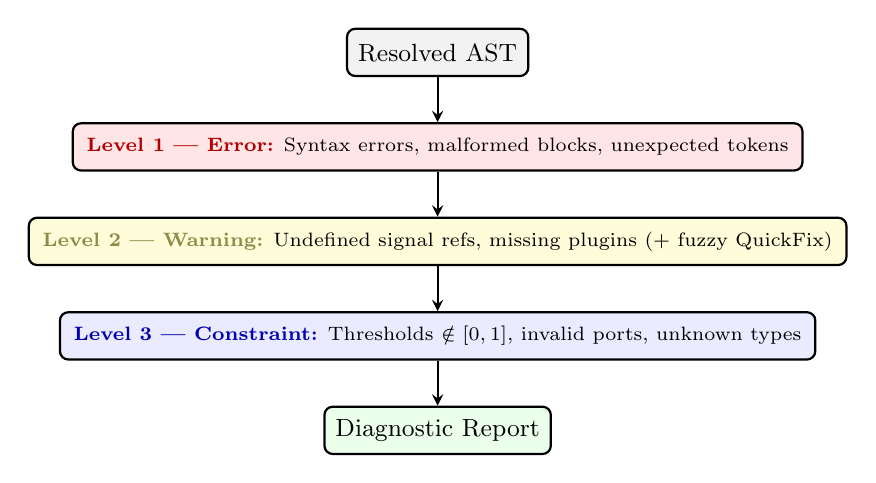
\begin{tikzpicture}[
    box/.style={rectangle, draw, thick, rounded corners=3pt,
                minimum height=0.6cm, minimum width=7.5cm, align=left, inner sep=5pt, font=\scriptsize},
    arr/.style={->, >=stealth, thick},
    lbl/.style={font=\scriptsize\bfseries},
  ]

  % AST input
  \node[rectangle, draw, thick, rounded corners=3pt, fill=black!5,
        minimum height=0.6cm, align=center, inner sep=4pt, font=\small] (ast) at (0, 3.6) {Resolved AST};

  % Level 1
  \node[box, fill=red!10] (l1) at (0, 2.4)
    {\textcolor{red!70!black}{\textbf{Level 1 --- Error:}} Syntax errors, malformed blocks, unexpected tokens};

  % Level 2
  \node[box, fill=yellow!15] (l2) at (0, 1.2)
    {\textcolor{yellow!50!black}{\textbf{Level 2 --- Warning:}} Undefined signal refs, missing plugins (+ fuzzy QuickFix)};

  % Level 3
  \node[box, fill=blue!8] (l3) at (0, 0)
    {\textcolor{blue!70!black}{\textbf{Level 3 --- Constraint:}} Thresholds $\notin [0,1]$, invalid ports, unknown types};

  \draw[arr] (ast) -- (l1);
  \draw[arr] (l1) -- (l2);
  \draw[arr] (l2) -- (l3);

  % Output
  \node[rectangle, draw, thick, rounded corners=3pt, fill=green!8,
        minimum height=0.6cm, align=center, inner sep=4pt, font=\small] (out) at (0, -1.2) {Diagnostic Report};
  \draw[arr] (l3) -- (out);

  \end{tikzpicture}%
}
  \caption{Three-level validation architecture. The validator processes the resolved AST through progressively deeper analysis: syntactic errors (Level~1), reference resolution with fuzzy-matched QuickFix suggestions (Level~2), and semantic constraint checking (Level~3). Diagnostics at all levels are accumulated into a unified report.}
  \label{fig:validation_levels}
\end{figure}

\subsection{DSL as Instruction Set and Agent-Based Policy Synthesis}
\label{sec:disc_agent}

The configuration language can be understood as the \emph{instruction set} of the neural-symbolic inference engine.
Just as a CPU's instruction set defines the space of programs that can execute on the hardware, the DSL defines the space of routing policies that can be instantiated on the signal-decision-plugin architecture.
The functional completeness result of \Cref{sec:decision_engine} guarantees that this instruction set is \emph{universal}: any routing policy $\pi: \{0,1\}^N \to \mathcal{M}$ is expressible.

This framing transforms the problem of \emph{configuring} the router into a \emph{program synthesis} problem (\Cref{fig:agent_synthesis}): given a natural-language specification of routing requirements (``route math queries to the math model, enforce PII filtering for healthcare queries''), synthesize a valid DSL configuration that implements the specification.
This is precisely the class of problems that code-generation agents---LLMs fine-tuned or prompted for program synthesis---are designed to solve.

The DSL's formal grammar and type-safe compilation make it particularly suitable as the target language: the structured syntax---with explicit keywords, typed blocks, and a finite set of signal types---constrains the generation space far more tightly than free-form YAML, reducing the probability of syntactically valid but semantically incorrect configurations.
The three-level validator provides immediate, machine-readable feedback that a coding agent can use to iteratively refine generated configurations.

\begin{figure*}[!ht]
  \centering
  \resizebox{\linewidth}{!}{%
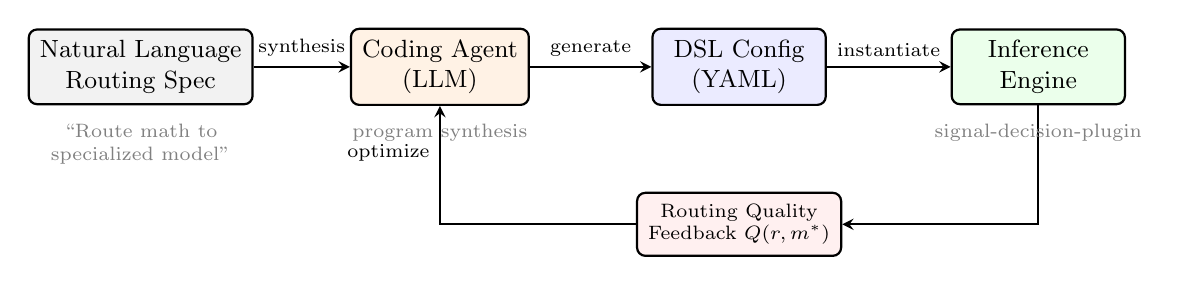
\begin{tikzpicture}[
    box/.style={rectangle, draw, thick, rounded corners=3pt,
                minimum height=0.8cm, align=center, inner sep=4pt, font=\small},
    arr/.style={->, >=stealth, thick},
    lbl/.style={font=\scriptsize, text=gray},
  ]

  % Natural language spec
  \node[box, fill=black!5, minimum width=2.2cm] (nl) at (0, 0) {Natural Language\\Routing Spec};

  % Coding Agent
  \node[box, fill=orange!10, minimum width=2.2cm] (agent) at (3.8, 0) {Coding Agent\\(LLM)};

  % DSL Config
  \node[box, fill=blue!8, minimum width=2.2cm] (dsl) at (7.6, 0) {DSL Config\\(YAML)};

  % Inference Engine
  \node[box, fill=green!8, minimum width=2.2cm] (engine) at (11.4, 0) {Inference\\Engine};

  % Feedback loop
  \node[box, fill=red!6, minimum width=2.0cm, font=\scriptsize] (fb) at (7.6, -2.0) {Routing Quality\\Feedback $Q(r, m^*)$};

  \draw[arr] (nl) -- node[above, font=\scriptsize] {synthesis} (agent);
  \draw[arr] (agent) -- node[above, font=\scriptsize] {generate} (dsl);
  \draw[arr] (dsl) -- node[above, font=\scriptsize] {instantiate} (engine);
  \draw[arr] (engine.south) |- (fb.east);
  \draw[arr] (fb.west) -| node[left, font=\scriptsize, pos=0.8] {optimize} (agent.south);

  % Labels
  \node[lbl, anchor=north] at (0, -0.6) {``Route math to};
  \node[lbl, anchor=north] at (0, -0.9) {specialized model''};
  \node[lbl, anchor=north] at (3.8, -0.6) {program synthesis};
  \node[lbl, anchor=north] at (11.4, -0.6) {signal-decision-plugin};

  \end{tikzpicture}%
}
  \caption{Agent-based policy synthesis pipeline. A coding agent (LLM) translates natural-language routing specifications into DSL configurations, which are instantiated on the inference engine. Routing quality feedback closes the loop, enabling iterative policy refinement. The DSL's functional completeness guarantees that any expressible routing policy is reachable by the synthesis process.}
  \label{fig:agent_synthesis}
\end{figure*}

The connection to reinforcement learning is direct: the coding agent's policy $\pi_\theta(\text{config} \mid \text{spec})$ can be optimized via RLHF or rule-based reward~\cite{zhang2025routerr1}, where the reward signal is the downstream routing quality $Q(r, m^*)$ aggregated over a traffic distribution.
This operates at a \emph{meta-level} compared to prior work on RL-based routing~\cite{zhang2025routerr1}: rather than learning to route individual requests, the agent learns to \emph{write routing policies} that generalize across request distributions.
The DSL provides the structured action space that makes this meta-learning tractable---the agent generates a finite, syntactically constrained configuration rather than an arbitrary neural network.

\subsection{Synthesis: A Programmable Neural-Symbolic Inference Engine}

Taken together, the signal extraction layer (\Cref{sec:signal_engine}), decision engine (\Cref{sec:decision_engine}), and configuration language characterize the system as a \textbf{programmable neural-symbolic inference engine}:

\begin{enumerate}
  \item \textbf{Neural front-end}: The signal extraction layer uses both heuristic and learned (neural) methods to produce a structured representation---analogous to a hybrid embedding layer (\Cref{sec:disc_embedding}).
  \item \textbf{Symbolic back-end}: The decision engine applies Boolean logic over the structured representation---analogous to symbolic expert gating with formal verifiability (\Cref{sec:disc_moe}).
  \item \textbf{Programmable interface}: The DSL configuration is the ``program'' that specifies the inference behavior, and the functional completeness of the Boolean decision model guarantees universality of the program space.
  \item \textbf{Agent-compilable}: The structured DSL enables LLM-based coding agents to serve as ``compilers'' from natural-language specifications to executable routing policies, with RL-based optimization closing the loop.
\end{enumerate}

This perspective unifies the Shannon-theoretic foundation (information reduction + Boolean synthesis) with the modern ML landscape (embeddings + MoE gating + agent-based program synthesis), and suggests that the architecture occupies a principled point in the design space between fully neural routing systems (which sacrifice interpretability and editability) and fully manual rule systems (which sacrifice adaptivity and scalability).

